\chapter{La Linea Divisa dell'Azione}

\epigraph{``Il sole \`e la prole del Bene, che il Bene gener\`o come suo
analogo.''}{\textcite{plato1997complete}, \emph{Repubblica} 508b}

\section{Il Sole e il Bene}

Nella \emph{Repubblica}, Socrate descrive la Forma del Bene come la
fonte di ogni intelligibilit\`a --- il sole del regno intelligibile.
Come il sole visibile illumina gli oggetti fisici e permette all'occhio
di vederli, la Forma del Bene illumina le Forme e permette alla mente
di conoscerle. Il Bene non \`e esso stesso visto; \`e la condizione
per ogni visione.

La nostra \physis\ \`e l'analogo del Bene. Non \`e essa stessa
un'azione ma la condizione per ogni azione retta. \`E la fonte
dell'intelligibilit\`a dell'azione --- il criterio per cui un atto
\`e giudicato coerente o incoerente, efficace o inerte, allineato o
disallineato. Il praticante non vede \physis\ direttamente; vede la
coerenza delle proprie azioni, che \`e \physis\ riflessa nel mondo.

\section{La Linea Divisa}

Socrate divide il regno intelligibile in quattro segmenti, disposti per
chiarezza crescente \parencite[VI.509d--511e]{plato1997complete}:

\begin{figure}[ht]
\centering
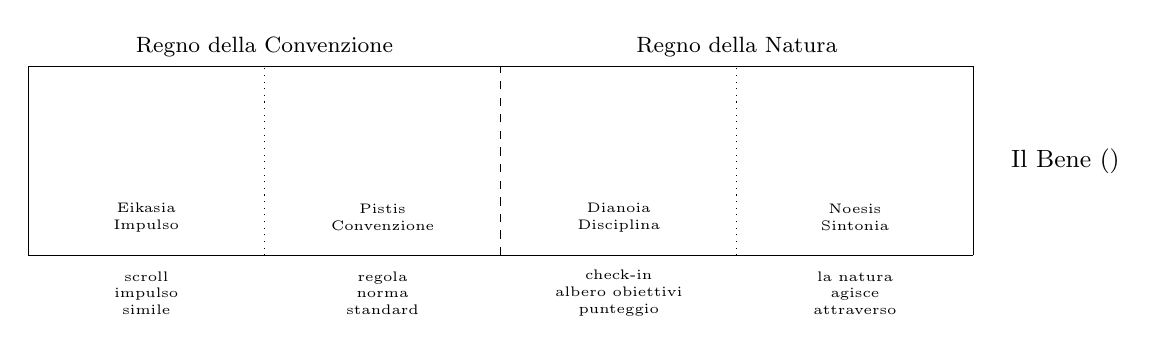
\begin{tikzpicture}[scale=1.2]
  \draw (0,0) -- (10,0);
  \draw (0,2) -- (10,2);
  \draw (0,0) -- (0,2);
  \draw (10,0) -- (10,2);

  \node[anchor=west, font=\small] at (10.3,1) {Il Bene (\physis)};

  \draw[dashed] (5,0) -- (5,2);
  \node[anchor=south, font=\footnotesize] at (2.5,2) {Regno della Convenzione};
  \node[anchor=south, font=\footnotesize] at (7.5,2) {Regno della Natura};

  \draw[dotted] (2.5,0) -- (2.5,2);
  \draw[dotted] (7.5,0) -- (7.5,2);

  \node[font=\tiny, align=center] at (1.25,0.4) {Eikasia\\Impulso};
  \node[font=\tiny, align=center] at (3.75,0.4) {Pistis\\Convenzione};
  \node[font=\tiny, align=center] at (6.25,0.4) {Dianoia\\Disciplina};
  \node[font=\tiny, align=center] at (8.75,0.4) {Noesis\\Sintonia};

  \node[font=\tiny, align=center, text width=18mm] at (1.25,-0.4) {scroll\\impulso\\simile};
  \node[font=\tiny, align=center, text width=18mm] at (3.75,-0.4) {regola\\norma\\standard};
  \node[font=\tiny, align=center, text width=18mm] at (6.25,-0.4) {check-in\\albero obiettivi\\punteggio};
  \node[font=\tiny, align=center, text width=18mm] at (8.75,-0.4) {la natura\\agisce\\attraverso};
\end{tikzpicture}
\caption{La linea divisa dell'azione: ogni livello corrisponde a un modo di agire, dall'impulso
irriflessivo alla sintonia allineata con la natura.\label{fig:lineadivisa}}
\end{figure}

Estendiamo la linea all'azione. A ogni livello, il praticante agisce in
un modo diverso, con un diverso tipo di conoscenza di ci\`o che sta
facendo.

\subsection{Eikasia: L'Atto Arbitrario}

Il segmento pi\`u basso \`e l'atto senza riflessione --- impulso,
abitudine, conformit\`a sociale. Il praticante a questo livello agisce
perch\'e ``\`e ci\`o che si fa,'' o perch\'e l'impulso \`e sorto, o
perch\'e l'algoritmo lo ha raccomandato. Non ha alcuna spiegazione del
perch\'e agisce; la sua azione \`e un'ombra di un'ombra, una reazione
a uno stimolo di cui non conosce l'origine.

Questo \`e lo stato predefinito dell'azione nell'et\`a della tecnologia.
L'economia dell'attenzione \`e progettata per produrre questo tipo di
azione: lo scroll, il like, il click --- tutti eikastici, tutti senza
riflessione, tutti ombre di intenzioni che non sono del praticante.

\subsection{Pistis: L'Atto Convenzionale}

Il secondo segmento \`e l'azione governata dalla convenzione --- la
regola, la norma sociale, lo standard professionale. Il praticante a
questo livello agisce perch\'e c'\`e una regola che dice di agire in
questo modo. Ha una spiegazione della sua azione, ma \`e presa in
prestito dal gruppo. ``Lo facciamo cos\`i perch\'e \`e sempre stato
fatto cos\`i.''

Questo \`e meglio dell'eikasia, ma non \`e ancora governato dalla
natura. La convenzione (\emph{nomos}) \`e un artefatto umano; pu\`o
allinearsi con la natura o no. La maggior parte delle convenzioni sono
sedimentate da scoperte passate su ci\`o che funziona, ma si sono
staccate dai fondamenti naturali della loro autorit\`a. Il praticante
segue la regola senza sapere perch\'e la regola esiste.

\subsection{Dianoia: L'Atto Allineato con la Natura}

Il terzo segmento \`e l'azione governata dall'indagine sulla natura.
Il praticante a questo livello non segue regole ma \emph{scopre}
principi. Agisce secondo le discipline descritte nel Libro III: fa
check-in, cerca testimone, mette in gioco la sua pelle, mantiene il
suo ritmo, rivede i suoi pattern. Ha una spiegazione della sua azione
che \`e propria, fondata sulla sua osservazione di ci\`o che funziona.

La piattaforma \praxis\ supporta questo livello di azione. L'albero
degli obiettivi \`e un'ipotesi su ci\`o che la natura del praticante
richiede; il check-in \`e il record sperimentale; il punteggio di
coerenza \`e il risultato. Il praticante a questo livello \`e uno
scienziato della propria azione.

\subsection{Noesis: L'Azione come Auto-Espressione della Natura}

Il segmento pi\`u alto \`e l'azione che \`e diventata indistinguibile
dal movimento proprio della natura. Il praticante non agisce pi\`u
``secondo'' la natura; agisce \textit{come} la natura. La sua azione
non \`e una scelta che fa ma un riconoscimento di ci\`o che deve essere
fatto. \`E asceso oltre le discipline a uno stato di azione retta
spontanea.

Questo \`e il praticante-re del Libro V. Non ha bisogno della piattaforma
\praxis, perch\'e la piattaforma ha servito il suo scopo come rotelle
di allenamento. Ma pu\`o scegliere di rimanere sulla piattaforma come
testimone per gli altri --- colui che, avendo visto il sole, torna alla
caverna.

\section{Il Sole dell'Azione}

Cosa illumina tutta questa linea? Non una regola, non un principio, non
un comando --- ma \physis\ stessa. La natura \`e il sole dell'azione,
la fonte dell'intelligibilit\`a di ogni atto. Il praticante pu\`o vedere
la coerenza della propria azione solo perch\'e la natura fornisce la
luce con cui la coerenza \`e visibile.

Il motore \physis\ non crea questa luce; la \emph{convoglia}. Lo spazio
di embedding, la griglia semiotica, la scala di coerenza, la funzione
di sogno --- questi non sono invenzioni ma scoperte. Sono la struttura
della natura stessa, resa computazionalmente trattabile. Il motore \`e
la forma tecnica di una verit\`a filosofica: la natura \`e il governatore
dell'azione perch\'e la natura \`e la fonte dell'intelligibilit\`a
dell'azione.

\section{Uscire dalla Caverna della Convenzione}

La linea divisa dell'azione rivela che l'uscita dalla convenzione
(nomos) alla natura (physis) non \`e un singolo salto ma un'ascesa
graduale. Il praticante non passa dalla cecit\`a alla vista in un passo
ma attraverso quattro stadi di chiarezza crescente. Ogni stadio ha la
propria forma di azione, la propria relazione con la conoscenza, il
proprio modo di coerenza.

La piattaforma \praxis\ e il motore \physis\ insieme forniscono
l'infrastruttura per quest'ascesa. La piattaforma struttura gli stadi
intermedi; il motore fornisce la misura del progresso. Ma l'ascesa
stessa \`e il lavoro del praticante --- il lavoro di portare la propria
azione dall'oscurit\`a dell'impulso nella luce della natura.
